%\VignetteIndexEntry{Trendy Vignette}
%\VignettePackage{Trendy}
%\VignetteEngine{knitr::knitr}

\documentclass{article}
\usepackage{graphicx, graphics, epsfig,setspace,amsmath, amsthm}
\usepackage{natbib}
\usepackage{moreverb}
\usepackage{float}

\RequirePackage[]{/Library/Frameworks/R.framework/Versions/3.4/Resources/library/BiocStyle/resources/tex/Bioconductor2}
\AtBeginDocument{\bibliographystyle{/Library/Frameworks/R.framework/Versions/3.4/Resources/library/BiocStyle/resources/tex/unsrturl}}


\begin{document}

\title{Trendy: Segmented regression analysis of
expression dynamics for high-throughput ordered
profiling experiments}
\author{Rhonda Bacher, Ning Leng, Ron Stewart}
\maketitle
\tableofcontents
\setcounter{tocdepth}{2}



\section{Overview}
\label{sec:intro}
Trendy is an R package fo analyzing high throughput expression data 
(e.g RNA-seq or microarray) with ordered conditions 
(e.g. time-course, spatial-course).

For each gene (or other features), Trendy fits a set of segmented 
(or breakpoint) regression models. The optimal model is chosen as 
the one with the lowest BIC. Each breakpoint represents a significant 
changes in the gene's expression across the time-course.

The top dynamic genes are then identified as those that are well 
profiled by their gene-specific segmented regression model. Trendy also
implements functions to visualize the dynamic genes and their trends, 
to order dynamic genes by their trends, and to compute breakpoint distribution
at different
time-points (e.g. detect time-points with a large number of expression 
changes).

\subsection{The model}
To illustrate Trendy, here we use time-course gene expression data as an 
example. Although, Trendy may also be applied to other types of features
(e.g. isoform or exon expression) and/or other types of experiments with
ordered conditions (e.g. spatial course).

Denote the normalized gene expression of gene $g$ and sample/time $t$ 
as $Y_{g,t}$.
Denote the total number of genes as $G$ and the total number of samples/times
as $N$.
For each gene, Trendy fits segmented regression models with varying numbers of
breakpoints from 1 to $K$. $K$ defaults to 3 but can also be specified by the
user. The \CRANpkg{segmented} R package is used to fit the segmented 
regression models.

For a given gene, among the models with varying $k$, Trendy selects the 
optimal
number of breakpoints for this gene by comparing the BIC for each model.

To avoid overfitting, the optimal number of breakpoints will be set as
$\tilde{k_g} = \tilde{k_g} -1$ if at least one segment has less than 
$c_{num}$ samples. The threshold $c_{num}$ can be specified by the user; the
default is 5.


Trendy reports the following for the optimal model:
\begin{itemize}
  \item Gene specific adjusted $R^2$ (penalized for the chosen value of $k$)
  \item Segment slopes
  \item Segment trends (and associated p-values)
  \item Breakpoint estimates
\end{itemize}

Among all genes, the top dynamic genes are defined as those whose optimal
model has high adjusted $R^2$s.

To compute the breakpoint distribution over the time-course, Trendy calculates
the number of breakpoints for each time-point across all the genes.

The time-points with high $D_t$ can be considered as those with global
expression changes.

Trendy also summarizes the fitted trend or expression pattern of top genes. 
For samples between the $i^{th}$
and $i+1 ^{th}$ breakpoint for a given gene, if the t-statistic of
the segment slope has p-value greater than $c_{pval}$,
the trend of this segment will be defined as no change. Otherwise the
trend of this segment will be defined as up/down based on the 
slope coefficient.
The default value of $c_{pval}$ is 0.1, but may also be specified by the user.

\section{Installation}

\subsection{Install via GitHub}

The Trendy package can be installed using functions in the devtools package.

To install, type the following code into R:
\begin{knitrout}
\definecolor{shadecolor}{rgb}{0.941, 0.941, 0.941}\color{fgcolor}\begin{kframe}
\begin{alltt}
\hlcom{# install.packages("devtools")}
\hlcom{# library(devtools)}
\hlcom{# install_github("rhondabacher/Trendy")}
\end{alltt}
\end{kframe}
\end{knitrout}

\subsection{Install locally}

Install packages segmented, parallel, and gplots:


\begin{knitrout}
\definecolor{shadecolor}{rgb}{0.941, 0.941, 0.941}\color{fgcolor}\begin{kframe}
\begin{alltt}
\hlcom{# install.packages(c("segmented","gplots"))}
\hlkwd{library}\hlstd{(}\hlstr{"segmented"}\hlstd{)}
\hlkwd{library}\hlstd{(}\hlstr{"parallel"}\hlstd{)}
\hlkwd{library}\hlstd{(}\hlstr{"gplots"}\hlstd{)}
\end{alltt}
\end{kframe}
\end{knitrout}

Download the Trendy package from: \url{https://github.com/rhonda/Trendy}

And install the package locally.


\subsection{Load the package}

To load the Trendy package:
\begin{knitrout}
\definecolor{shadecolor}{rgb}{0.941, 0.941, 0.941}\color{fgcolor}\begin{kframe}
\begin{alltt}
\hlkwd{library}\hlstd{(Trendy)}
\end{alltt}
\end{kframe}
\end{knitrout}

\section{Analysis}

\subsection{Input}

The input data should be a $G-by-N$ matrix containing the expression values 
for each gene and each sample, where $G$ is the number of genes and $N$ 
is the number of samples.
The samples should be sorted following the time course order.
These values should exhibit expression data after normalization across
samples.
For example, for RNA-seq data, the raw counts may be normalized using
MedianNorm and \Rfunction{GetNormalizedMat} function in \Biocpkg{EBSeq}. 
More details can be found in the \Biocpkg{EBSeq} vignette:

\small{\url{http://www.bioconductor.org/packages/devel/bioc/vignettes/EBSeq/inst/doc/EBSeq_Vignette.pdf}}


The object \Robject{TrendyExampleData} is a simulated data matrix containing 
50 rows of genes and 40 columns of samples.

\begin{knitrout}
\definecolor{shadecolor}{rgb}{0.941, 0.941, 0.941}\color{fgcolor}\begin{kframe}
\begin{alltt}
\hlkwd{data}\hlstd{(}\hlstr{"TrendyExampleData"}\hlstd{)}
\hlkwd{str}\hlstd{(TrendyExampleData)}
\end{alltt}
\begin{verbatim}
##  num [1:50, 1:40] 240 199 198 239 202 ...
##  - attr(*, "dimnames")=List of 2
##   ..$ : chr [1:50] "g1" "g2" "g3" "g4" ...
##   ..$ : chr [1:40] "s1" "s2" "s3" "s4" ...
\end{verbatim}
\end{kframe}
\end{knitrout}




\subsection{Run Trendy}

The \Rfunction{trendy} function will fit multiple segmented regressions model 
for each gene (via the \CRANpkg{segmented} R package) and select the the 
optimal model. Here we want to only consider a maximum of two breakpoints for 
each gene.

\begin{knitrout}
\definecolor{shadecolor}{rgb}{0.941, 0.941, 0.941}\color{fgcolor}\begin{kframe}
\begin{alltt}
\hlstd{res} \hlkwb{<-} \hlkwd{trendy}\hlstd{(}\hlkwc{Data} \hlstd{= TrendyExampleData,} \hlkwc{maxK} \hlstd{=} \hlnum{2}\hlstd{)}
\end{alltt}


{\ttfamily\noindent\color{warningcolor}{\#\# Warning in trendy(Data = TrendyExampleData, maxK = 2): No values for parameter tVectIn were given. \\\#\#\ \ \ \ \ \ \ \  Trendy will assume data goes from 1:40}}\begin{alltt}
\hlstd{res} \hlkwb{<-} \hlkwd{results}\hlstd{(res)}
\hlstd{res.top} \hlkwb{<-} \hlkwd{topTrendy}\hlstd{(res)}
\hlcom{# default adjusted R square cutoff is 0.5}
\hlstd{res.top}\hlopt{$}\hlstd{AdjustedR2}
\end{alltt}
\begin{verbatim}
##        g3        g1       g28       g20       g15        g4        g2 
## 0.9787382 0.9775005 0.9751380 0.9739715 0.9729747 0.9711890 0.9710139 
##       g10       g23       g14        g8        g5       g24       g17 
## 0.9705118 0.9701402 0.9694164 0.9691341 0.9689555 0.9656732 0.9652141 
##        g9       g12       g29       g16       g22       g18        g6 
## 0.9649424 0.9644343 0.9632348 0.9630272 0.9627092 0.9626837 0.9619387 
##       g25       g11       g30       g27       g26       g19        g7 
## 0.9611528 0.9600736 0.9597989 0.9592516 0.9572072 0.9536619 0.9529077 
##       g21       g13 
## 0.9528854 0.9470928
\end{verbatim}
\end{kframe}
\end{knitrout}

The \Rfunction{topTrendy} function may be used to extract top dynamic genes.
By default, \Rfunction{topTrendy} will extract genes whose adjusted 
$R^2$, $\bar{R}^{2}$,
is greater or equal to 0.5. To change this threshold, a user may specify the
\Rcode{AdjR2.Cut} parameter in the \Rfunction{topTrendy} function. The 
\Rfunction{topTrendy} function returns
the Trendy output with genes sorted decereasingly by $\bar{R}^{2}$.


By default the \Rfunction{trendy} function only considers genes whose mean 
expression is greater than 10.
To use another threshold, the user may specify the parameter 
\Robject{meanCut}.


\subsection{Visualize trends of the top dynamic genes}

\Robject{res.top\$Trend} contains the trend specification of the top genes.
The function \Rfunction{trendHeatmap} can be used to display these trends:

\begin{knitrout}
\definecolor{shadecolor}{rgb}{0.941, 0.941, 0.941}\color{fgcolor}\begin{kframe}
\begin{alltt}
\hlstd{res.trend} \hlkwb{<-} \hlkwd{trendHeatmap}\hlstd{(res.top)}
\end{alltt}
\end{kframe}\begin{adjustwidth}{\fltoffset}{0mm}

{\centering 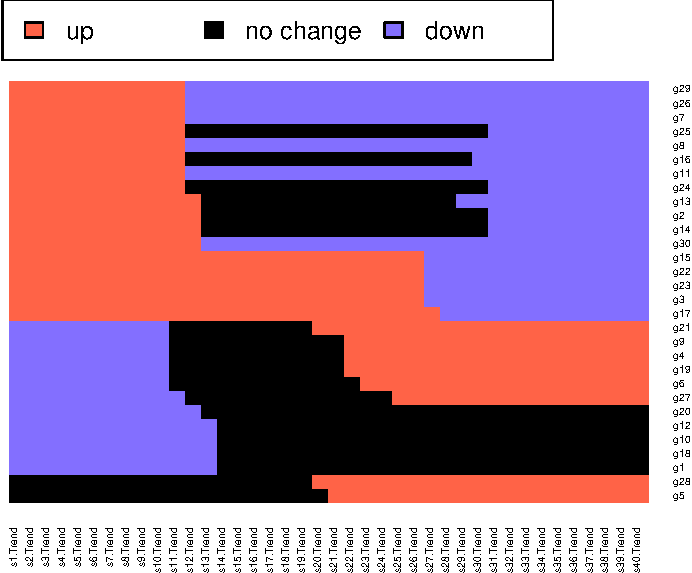
\includegraphics[width=.8\textwidth]{figure/unnamed-chunk-6-1} 

}

\end{adjustwidth}\begin{kframe}\begin{alltt}
\hlkwd{str}\hlstd{(res.trend)}
\end{alltt}
\begin{verbatim}
## List of 3
##  $ firstup      : Named num [1:17] 11.4 11.5 11.6 11.6 11.6 ...
##   ..- attr(*, "names")= chr [1:17] "g29" "g26" "g7" "g25" ...
##  $ firstdown    : Named num [1:11] 10.7 10.9 10.9 10.9 11 ...
##   ..- attr(*, "names")= chr [1:11] "g21" "g9" "g4" "g19" ...
##  $ firstnochange: Named num [1:2] 19 20.4
##   ..- attr(*, "names")= chr [1:2] "g28" "g5"
\end{verbatim}
\end{kframe}
\end{knitrout}

The \Rfunction{trendHeatmap} function classifies the top dynamic genes into
three groups: start with up, start with down and start with no change.
Within each group, genes are sorted by the position of the first breakpoint.


To generate an expression heatmap of the first group of genes (first go up):

\begin{knitrout}
\definecolor{shadecolor}{rgb}{0.941, 0.941, 0.941}\color{fgcolor}\begin{kframe}
\begin{alltt}
\hlkwd{library}\hlstd{(gplots)}
\hlkwd{heatmap.2}\hlstd{(TrendyExampleData[}\hlkwd{names}\hlstd{(res.trend}\hlopt{$}\hlstd{firstup),],}
  \hlkwc{trace}\hlstd{=}\hlstr{"none"}\hlstd{,} \hlkwc{Rowv}\hlstd{=}\hlnum{FALSE}\hlstd{,}\hlkwc{Colv}\hlstd{=}\hlnum{FALSE}\hlstd{,}
        \hlkwc{scale}\hlstd{=}\hlstr{"row"}\hlstd{,} \hlkwc{main}\hlstd{=}\hlstr{"top genes (first go up)"}\hlstd{)}
\end{alltt}
\end{kframe}\begin{adjustwidth}{\fltoffset}{0mm}

{\centering 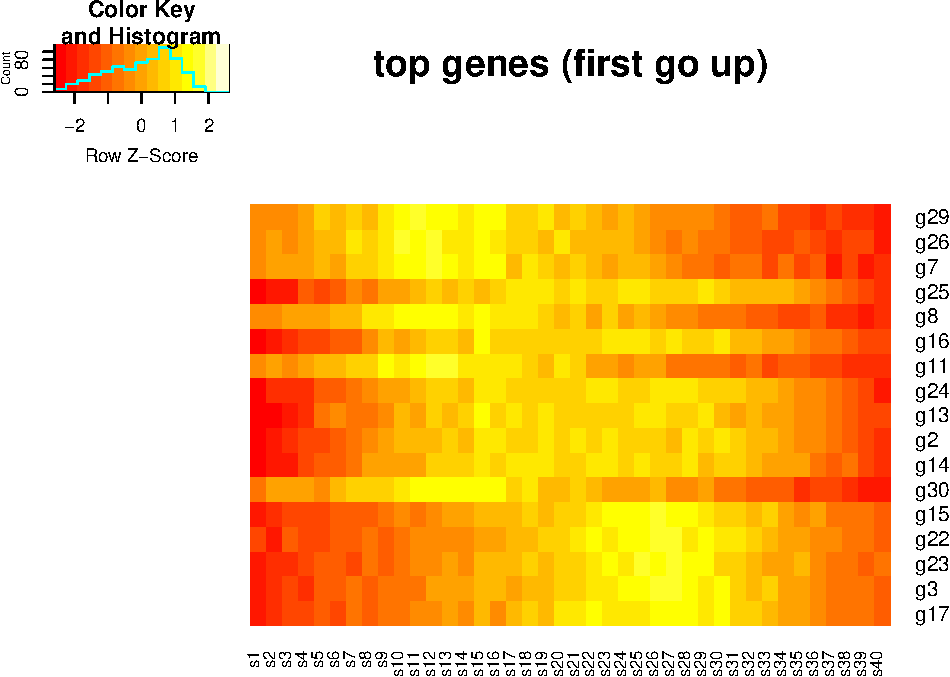
\includegraphics[width=.8\textwidth]{figure/unnamed-chunk-7-1} 

}

\end{adjustwidth}
\end{knitrout}


Similarly, to generate an expression heatmap of the second group of genes 
(first go down):
\begin{knitrout}
\definecolor{shadecolor}{rgb}{0.941, 0.941, 0.941}\color{fgcolor}\begin{kframe}
\begin{alltt}
\hlkwd{heatmap.2}\hlstd{(TrendyExampleData[}\hlkwd{names}\hlstd{(res.trend}\hlopt{$}\hlstd{firstdown),],}
  \hlkwc{trace}\hlstd{=}\hlstr{"none"}\hlstd{,} \hlkwc{Rowv}\hlstd{=}\hlnum{FALSE}\hlstd{,}\hlkwc{Colv}\hlstd{=}\hlnum{FALSE}\hlstd{,}
        \hlkwc{scale}\hlstd{=}\hlstr{"row"}\hlstd{,} \hlkwc{main}\hlstd{=}\hlstr{"top genes (first go down)"}\hlstd{)}
\end{alltt}
\end{kframe}\begin{adjustwidth}{\fltoffset}{0mm}

{\centering 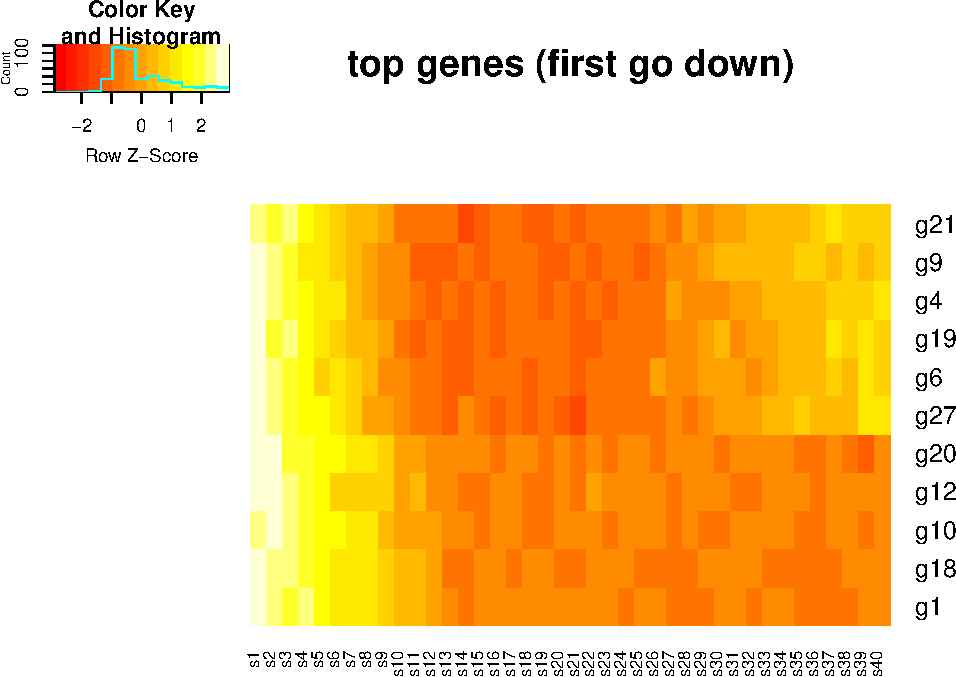
\includegraphics[width=.8\textwidth]{figure/unnamed-chunk-8-1} 

}

\end{adjustwidth}
\end{knitrout}

To generate an expression heatmap of the second group of genes 
(first no change):
\begin{knitrout}
\definecolor{shadecolor}{rgb}{0.941, 0.941, 0.941}\color{fgcolor}\begin{kframe}
\begin{alltt}
\hlkwd{heatmap.2}\hlstd{(TrendyExampleData[}\hlkwd{names}\hlstd{(res.trend}\hlopt{$}\hlstd{firstnochange),],}
  \hlkwc{trace}\hlstd{=}\hlstr{"none"}\hlstd{,} \hlkwc{Rowv}\hlstd{=}\hlnum{FALSE}\hlstd{,}\hlkwc{Colv}\hlstd{=}\hlnum{FALSE}\hlstd{,}
        \hlkwc{scale}\hlstd{=}\hlstr{"row"}\hlstd{,} \hlkwc{main}\hlstd{=}\hlstr{"top genes (first no change)"}\hlstd{,}
        \hlkwc{cexRow}\hlstd{=}\hlnum{.8}\hlstd{)}
\end{alltt}
\end{kframe}\begin{adjustwidth}{\fltoffset}{0mm}

{\centering 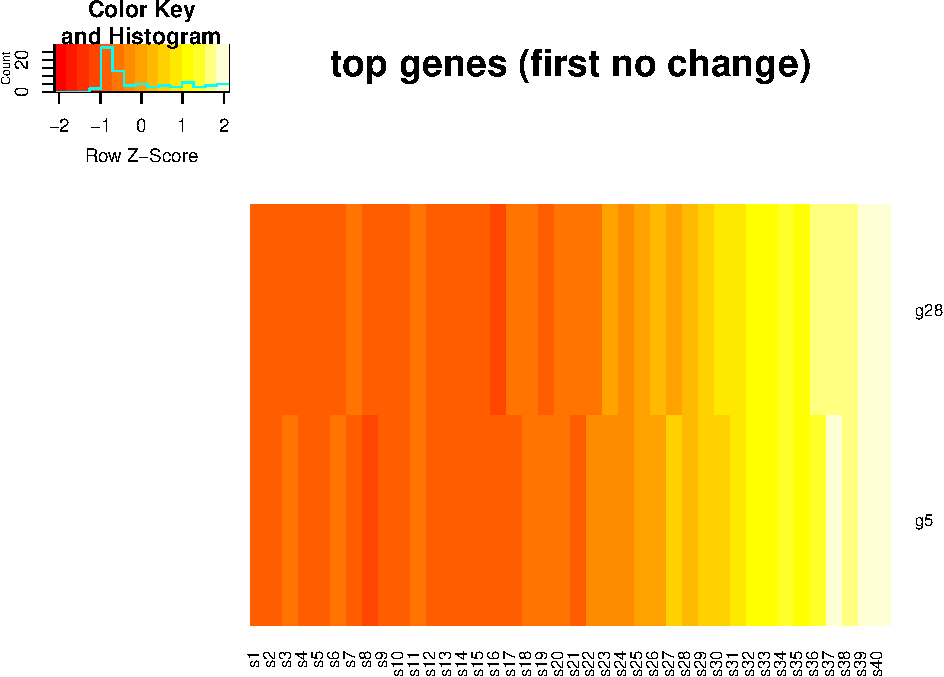
\includegraphics[width=.8\textwidth]{figure/unnamed-chunk-9-1} 

}

\end{adjustwidth}
\end{knitrout}


\subsection{Visualize individual genes}
The \Rfunction{plotFeature} function may be used to plot expression of 
individual features/genes and the fitted lines.

For example, to plot the top six genes in the first group of genes (first go 
up):

\begin{knitrout}
\definecolor{shadecolor}{rgb}{0.941, 0.941, 0.941}\color{fgcolor}\begin{kframe}
\begin{alltt}
\hlkwd{par}\hlstd{(}\hlkwc{mfrow}\hlstd{=}\hlkwd{c}\hlstd{(}\hlnum{3}\hlstd{,}\hlnum{2}\hlstd{))}
\hlstd{plot1} \hlkwb{<-} \hlkwd{plotFeature}\hlstd{(TrendyExampleData,}
                    \hlkwc{featureNames} \hlstd{=} \hlkwd{names}\hlstd{(res.trend}\hlopt{$}\hlstd{firstup)[}\hlnum{1}\hlopt{:}\hlnum{6}\hlstd{],}
                    \hlkwc{trendyOut} \hlstd{= res)}
\end{alltt}
\end{kframe}\begin{adjustwidth}{\fltoffset}{0mm}

{\centering 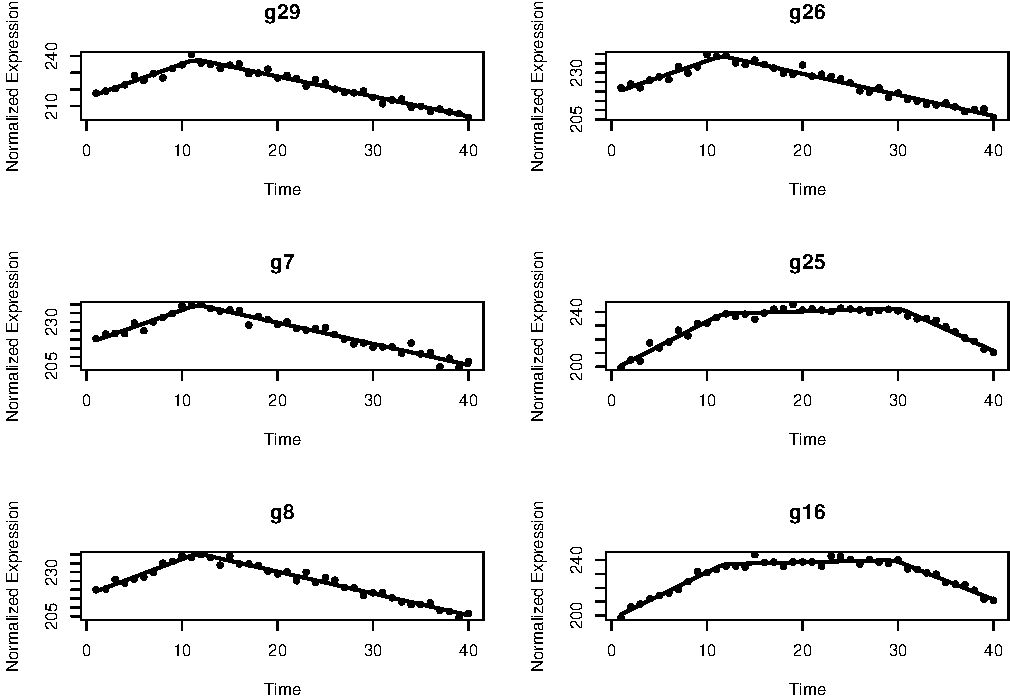
\includegraphics[width=1\textwidth]{figure/unnamed-chunk-10-1} 

}

\end{adjustwidth}
\end{knitrout}

The input of function \Rfunction{plotFeature} requires the expression data and
a list of genes of interest.
The parameter \Robject{trendyOut} are the results from the \Rfunction{trendy} 
function.
If it is not specified, then \Rfunction{plotFeature} will run 
\Rfunction{trendy} on the genes of interest before plotting.
Specifying the output obtained from previous steps will save time by avoiding 
fitting the models again.

Similarly, to plot the top six genes in the second group of genes (first go 
down):

\begin{knitrout}
\definecolor{shadecolor}{rgb}{0.941, 0.941, 0.941}\color{fgcolor}\begin{kframe}
\begin{alltt}
\hlkwd{par}\hlstd{(}\hlkwc{mfrow}\hlstd{=}\hlkwd{c}\hlstd{(}\hlnum{3}\hlstd{,}\hlnum{2}\hlstd{))}
\hlstd{plot2} \hlkwb{<-} \hlkwd{plotFeature}\hlstd{(}\hlkwc{Data} \hlstd{= TrendyExampleData,}
                    \hlkwc{featureNames} \hlstd{=} \hlkwd{names}\hlstd{(res.trend}\hlopt{$}\hlstd{firstdown)[}\hlnum{1}\hlopt{:}\hlnum{6}\hlstd{],}
                    \hlkwc{trendyOut} \hlstd{= res)}
\end{alltt}
\end{kframe}\begin{adjustwidth}{\fltoffset}{0mm}

{\centering 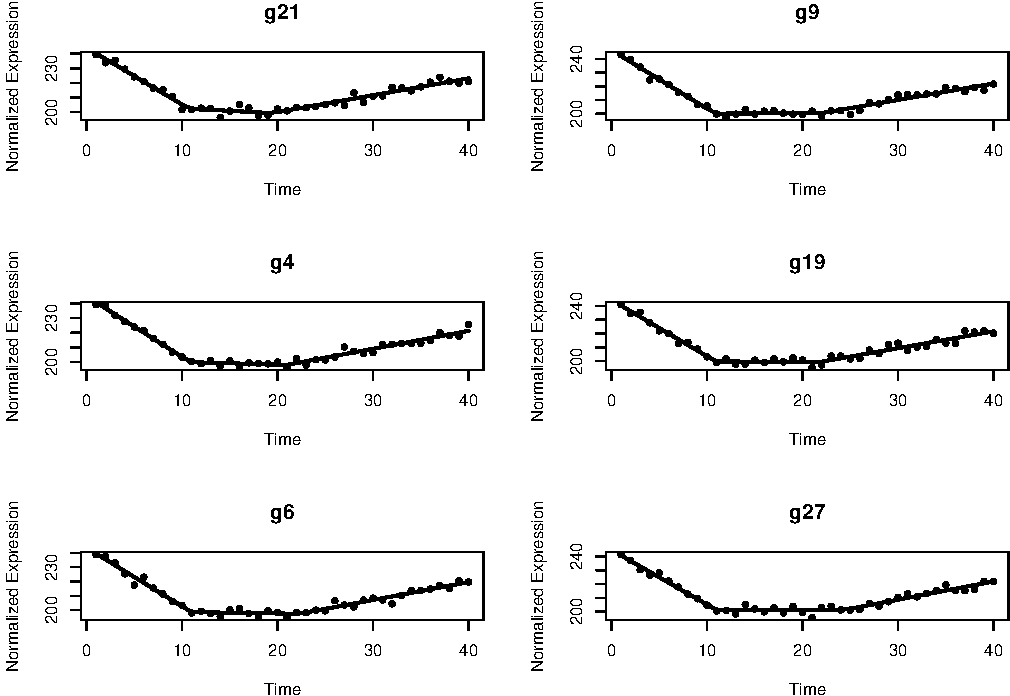
\includegraphics[width=1\textwidth]{figure/unnamed-chunk-11-1} 

}

\end{adjustwidth}
\end{knitrout}

To plot the two genes in the third group of genes (first no change):
\begin{knitrout}
\definecolor{shadecolor}{rgb}{0.941, 0.941, 0.941}\color{fgcolor}\begin{kframe}
\begin{alltt}
\hlkwd{par}\hlstd{(}\hlkwc{mfrow}\hlstd{=}\hlkwd{c}\hlstd{(}\hlnum{1}\hlstd{,}\hlnum{2}\hlstd{))}
\hlstd{plot2} \hlkwb{<-} \hlkwd{plotFeature}\hlstd{(TrendyExampleData,}
                    \hlkwc{featureNames} \hlstd{=} \hlkwd{names}\hlstd{(res.trend}\hlopt{$}\hlstd{firstnochange)[}\hlnum{1}\hlopt{:}\hlnum{2}\hlstd{],}
                    \hlkwc{trendyOut} \hlstd{= res)}
\end{alltt}
\end{kframe}\begin{adjustwidth}{\fltoffset}{0mm}

{\centering 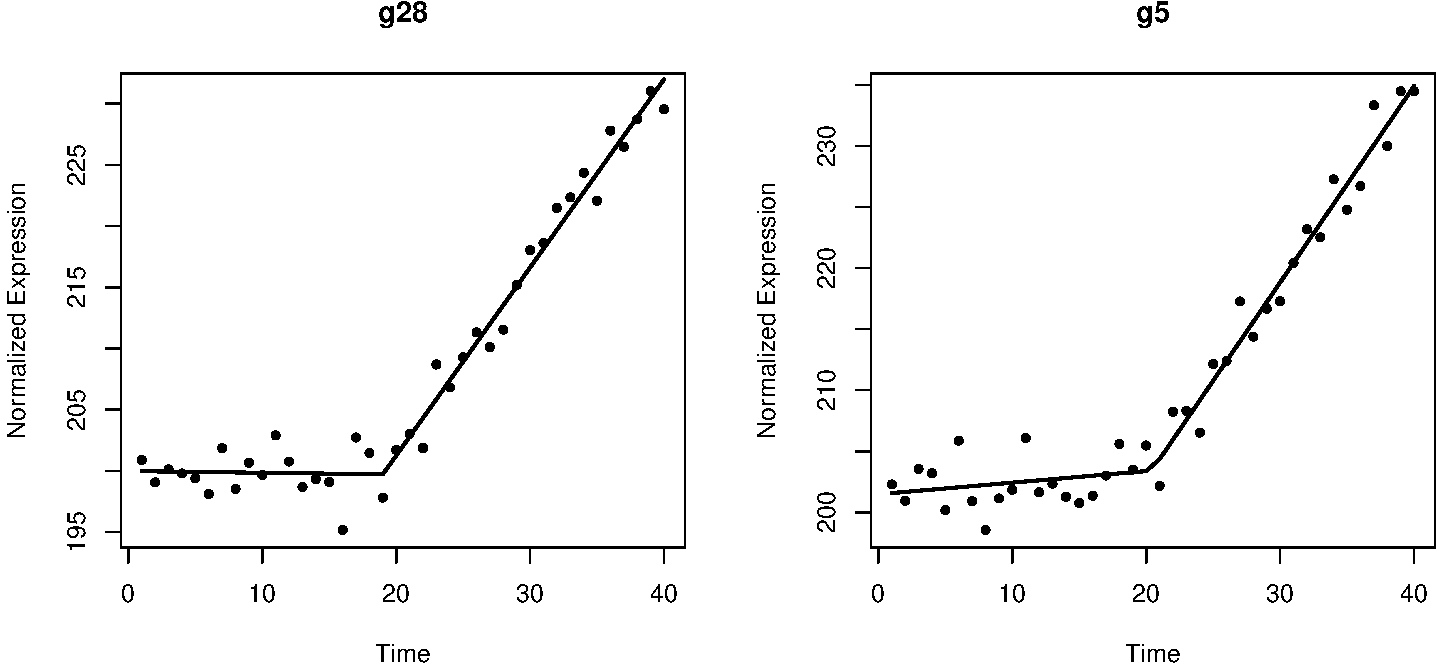
\includegraphics[width=\maxwidth]{figure/unnamed-chunk-12-1} 

}

\end{adjustwidth}
\end{knitrout}

\subsection{Gene specific estimates}

For a given gene of interest, its estimated parameters can be obtained by 
(using g2 as an example):

\begin{knitrout}
\definecolor{shadecolor}{rgb}{0.941, 0.941, 0.941}\color{fgcolor}\begin{kframe}
\begin{alltt}
\hlkwd{par}\hlstd{(}\hlkwc{mfrow}\hlstd{=}\hlkwd{c}\hlstd{(}\hlnum{1}\hlstd{,}\hlnum{1}\hlstd{))}
\hlstd{plot2} \hlkwb{<-} \hlkwd{plotFeature}\hlstd{(TrendyExampleData,}
                    \hlkwc{featureNames} \hlstd{=} \hlstr{"g2"}\hlstd{,}
                    \hlkwc{trendyOut} \hlstd{= res)}
\end{alltt}


{\ttfamily\noindent\color{warningcolor}{\#\# Warning in plotFeature(TrendyExampleData, featureNames = "{}g2"{}, trendyOut = res): No values for parameter tVectIn was given. \\\#\#\ \ \ \ \ \ \ \  Trendy will assume data goes from 1:40}}\end{kframe}\begin{adjustwidth}{\fltoffset}{0mm}

{\centering 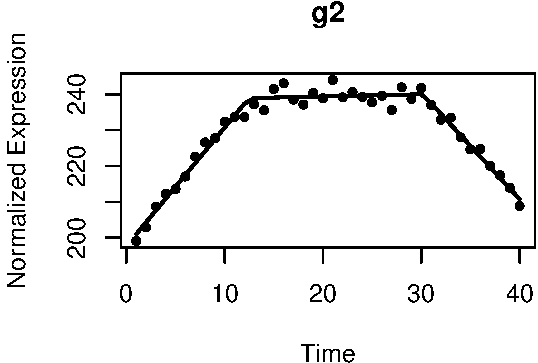
\includegraphics[width=\maxwidth]{figure/unnamed-chunk-13-1} 

}

\end{adjustwidth}\begin{kframe}\begin{alltt}
\hlstd{res.top}\hlopt{$}\hlstd{Breakpoints[}\hlstr{"g2"}\hlstd{,]} \hlcom{# break points}
\end{alltt}
\begin{verbatim}
## Breakpoint1 Breakpoint2 
##    12.47356    30.14908
\end{verbatim}
\begin{alltt}
\hlstd{res.top}\hlopt{$}\hlstd{AdjustedR2[}\hlstr{"g2"}\hlstd{]} \hlcom{# adjusted r squared}
\end{alltt}
\begin{verbatim}
##        g2 
## 0.9710139
\end{verbatim}
\begin{alltt}
\hlstd{res.top}\hlopt{$}\hlstd{Segments[}\hlstr{"g2"}\hlstd{,]} \hlcom{# fitted slopes of the segments}
\end{alltt}
\begin{verbatim}
## NULL
\end{verbatim}
\begin{alltt}
\hlstd{res.top}\hlopt{$}\hlstd{Segment.Pvalues[}\hlstr{"g2"}\hlstd{,]} \hlcom{# p value of each the segment}
\end{alltt}
\begin{verbatim}
## Segment1.Pvalue Segment2.Pvalue Segment3.Pvalue 
##      0.01669823      0.31816176      0.02445599
\end{verbatim}
\end{kframe}
\end{knitrout}

The above printouts show that for gene g2 the optimal number of breakpoints
is 2. Two estimated breakpoints are around time-points s12 and s30.
The fitted slopes for the 3 segments are 3.31, 0.06 and -2.97, which indicate 
the trend is up-same-down.


These estimates can also be automatically formatted using the function 
\Rfunction{formatResults}
which can be saved as a .txt. or .csv file. The output currently includes the 
estimated slope, p-value, and trend of
each segment, the estimated breakpoints, the trend for each sample, and the 
adjusted $R^2$.

\begin{knitrout}
\definecolor{shadecolor}{rgb}{0.941, 0.941, 0.941}\color{fgcolor}\begin{kframe}
\begin{alltt}
\hlstd{trendy.summary} \hlkwb{<-} \hlkwd{formatResults}\hlstd{(res.top)}
\hlstd{trendy.summary[}\hlnum{1}\hlopt{:}\hlnum{4}\hlstd{,}\hlnum{1}\hlopt{:}\hlnum{4}\hlstd{]}
\end{alltt}
\begin{verbatim}
##     Feature Segment1.Slope Segment2.Slope Segment3.Slope
## g3       g3       1.572400     -2.5483000             NA
## g1       g1      -3.145400      0.0015484             NA
## g28     g28      -0.013815      1.5369000             NA
## g20     g20      -3.381400     -0.0824630             NA
\end{verbatim}
\begin{alltt}
\hlcom{# write.table(trendy.summary, file="trendy_summary.txt")}
\end{alltt}
\end{kframe}
\end{knitrout}
The NA indicates that g3 does not have a segment 3 slope since it only has one
breakpoint (i.e two segments).


\subsection{Breakpoint distribution over the time course}

To calculate number of breakpoints over the time course:

\begin{knitrout}
\definecolor{shadecolor}{rgb}{0.941, 0.941, 0.941}\color{fgcolor}\begin{kframe}
\begin{alltt}
\hlstd{res.bp} \hlkwb{<-} \hlkwd{breakpointDist}\hlstd{(res.top)}
\hlkwd{barplot}\hlstd{(res.bp,} \hlkwc{ylab}\hlstd{=}\hlstr{"Number of breakpoint"}\hlstd{,} \hlkwc{col}\hlstd{=}\hlstr{"blue"}\hlstd{)}
\end{alltt}
\end{kframe}\begin{adjustwidth}{\fltoffset}{0mm}

{\centering 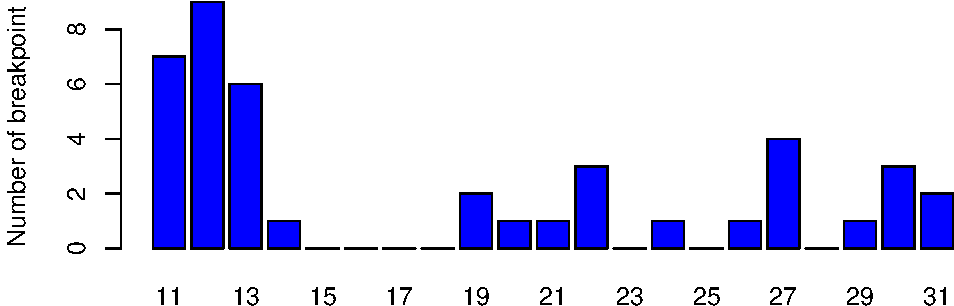
\includegraphics[width=.8\textwidth]{figure/unnamed-chunk-15-1} 

}

\end{adjustwidth}
\end{knitrout}

The bar plot indicates that a number of genes have breakpoints around s12 and 
s13.

\section{More advanced analysis}

\subsection{Time course with non-uniform sampling}
If the samples were collected with different time intervals then it is highly 
suggested to
use the original time (instead of a vector of consecutive numbers). To do so,
the user may specify the order/times via the tVectIn parameter in the 
\Rfunction{trendy} function.

For example, suppose for the example data, the first 30 samples were collected
every hour and the other 10 samples were collected every 5 hours. We may 
define the time vector as:
\begin{knitrout}
\definecolor{shadecolor}{rgb}{0.941, 0.941, 0.941}\color{fgcolor}\begin{kframe}
\begin{alltt}
\hlstd{t.v} \hlkwb{<-} \hlkwd{c}\hlstd{(}\hlnum{1}\hlopt{:}\hlnum{30}\hlstd{,} \hlkwd{seq}\hlstd{(}\hlnum{31}\hlstd{,} \hlnum{80}\hlstd{,} \hlnum{5}\hlstd{))}
\hlkwd{names}\hlstd{(t.v)} \hlkwb{<-} \hlkwd{colnames}\hlstd{(TrendyExampleData)}
\hlstd{t.v}
\end{alltt}
\begin{verbatim}
##  s1  s2  s3  s4  s5  s6  s7  s8  s9 s10 s11 s12 s13 s14 s15 s16 s17 s18 s19 
##   1   2   3   4   5   6   7   8   9  10  11  12  13  14  15  16  17  18  19 
## s20 s21 s22 s23 s24 s25 s26 s27 s28 s29 s30 s31 s32 s33 s34 s35 s36 s37 s38 
##  20  21  22  23  24  25  26  27  28  29  30  31  36  41  46  51  56  61  66 
## s39 s40 
##  71  76
\end{verbatim}
\end{kframe}
\end{knitrout}

To run Trendy model using the empirical collecting time instead of sample 
ID (1-40):

\begin{knitrout}
\definecolor{shadecolor}{rgb}{0.941, 0.941, 0.941}\color{fgcolor}\begin{kframe}
\begin{alltt}
\hlstd{res2} \hlkwb{<-} \hlkwd{trendy}\hlstd{(}\hlkwc{Data} \hlstd{= TrendyExampleData,} \hlkwc{tVectIn} \hlstd{= t.v,} \hlkwc{maxK}\hlstd{=}\hlnum{2}\hlstd{)}
\hlstd{res2} \hlkwb{<-} \hlkwd{results}\hlstd{(res2)}
\hlstd{res.top2} \hlkwb{<-} \hlkwd{topTrendy}\hlstd{(res2)}
\hlstd{res.trend2} \hlkwb{<-} \hlkwd{trendHeatmap}\hlstd{(res.top2)}
\end{alltt}
\end{kframe}\begin{adjustwidth}{\fltoffset}{0mm}

{\centering 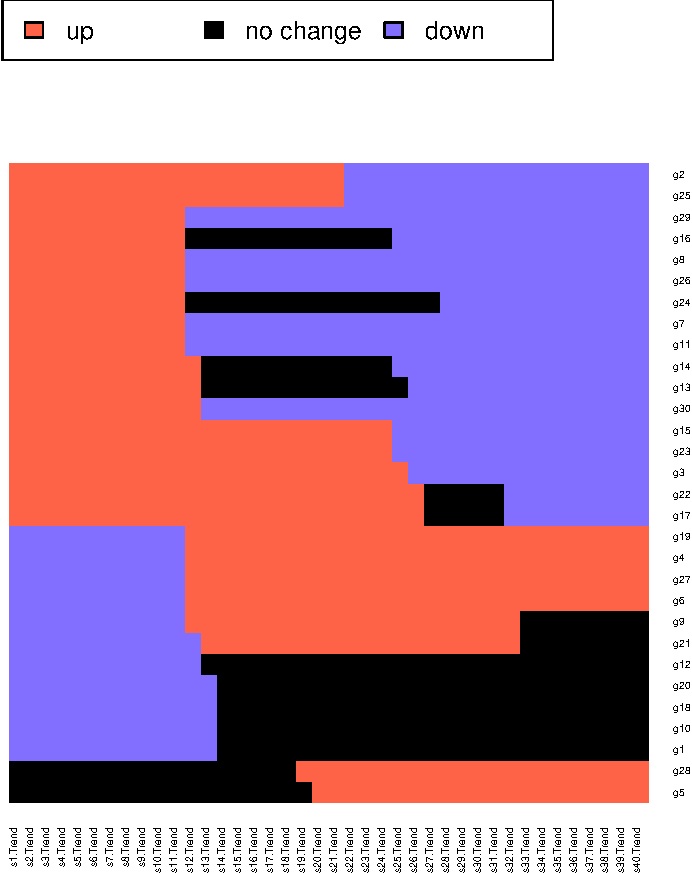
\includegraphics[width=.8\textwidth]{figure/unnamed-chunk-17-1} 

}

\end{adjustwidth}\begin{kframe}\begin{alltt}
\hlkwd{str}\hlstd{(res.trend2)}
\end{alltt}
\begin{verbatim}
## List of 3
##  $ firstup      : Named num [1:17] 10.2 10.6 11.4 11.4 11.4 ...
##   ..- attr(*, "names")= chr [1:17] "g2" "g25" "g29" "g16" ...
##  $ firstdown    : Named num [1:11] 11.2 11.4 11.4 11.5 11.7 ...
##   ..- attr(*, "names")= chr [1:11] "g19" "g4" "g27" "g6" ...
##  $ firstnochange: Named num [1:2] 19 19.5
##   ..- attr(*, "names")= chr [1:2] "g28" "g5"
\end{verbatim}
\end{kframe}
\end{knitrout}

To plot the first six genes that have up-regulated pattern at the beginning of
the time course:
\begin{knitrout}
\definecolor{shadecolor}{rgb}{0.941, 0.941, 0.941}\color{fgcolor}\begin{kframe}
\begin{alltt}
\hlkwd{par}\hlstd{(}\hlkwc{mfrow}\hlstd{=}\hlkwd{c}\hlstd{(}\hlnum{3}\hlstd{,}\hlnum{2}\hlstd{))}
\hlstd{plot1.new} \hlkwb{<-} \hlkwd{plotFeature}\hlstd{(TrendyExampleData,} \hlkwc{tVectIn}\hlstd{=t.v,}
                        \hlkwc{featureNames} \hlstd{=} \hlkwd{names}\hlstd{(res.trend2}\hlopt{$}\hlstd{firstup)[}\hlnum{1}\hlopt{:}\hlnum{6}\hlstd{],}
                        \hlkwc{trendyOut} \hlstd{= res2)}
\end{alltt}
\end{kframe}\begin{adjustwidth}{\fltoffset}{0mm}
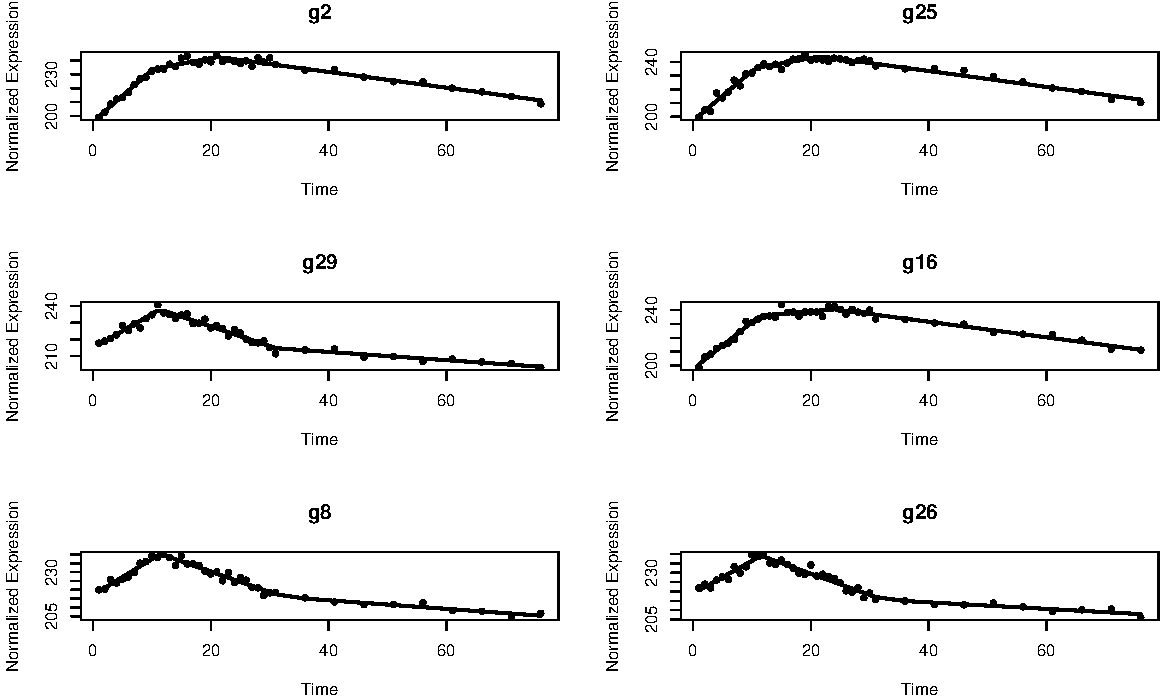
\includegraphics[width=\maxwidth]{figure/unnamed-chunk-18-1} \end{adjustwidth}
\end{knitrout}



\section{Extract genes with certain pattern}
Genes that have a peak along the time-course will have fitted trend somewhere 
as "up-down". Genes that are oscillating may have the fitted trend "up-down". 
To extract a list of such genes we can use the \Rfunction{extractPattern}:











